\subsection{GPU Acceleration}\label{section: gpu-acceleration}
The polynomial computations of ZK mainly consists of multiple NTTs and iNTTs. The large-size NTTs result in sigificant challenges for both off-chip memory accesses and on-chip compute resources, due to the irregular strided access patterns similar to classical FFTs. The GPU acceleration section takes full advantage of GPU multi-threaded parallel processing to speed up NTT calculations.
\subsubsection{NTT Computations}
The NTT computation is defined as
\[\hat{a} = NTT{(a)}\]
Where $a$ and  $\hat{a}$ are two $N$ size arrays, and  $\hat{a}[i] = \sum_{j=0}^{N-1} a[j] \omega_N^{ij}$. Here $a[i]$ and $\hat{a}[i]$ are $\lambda$-bit scalars in a finite field. And $\omega_N$ is the $N$-th root of unity in the same field, also is called twiddle factor, which is a constant value for a specific size of $N$.

Similar to classical FFTs, optimized and improved performance implementations of the NTT are of necessity and fundamental essentials. Cooley-Tukey processing is a commonly used NTT algorithm in science and engineering. For example, the Cooley-Tukey algorithm reduces the computational complexity from $O(N^2)$ to $O(N\log N)$. Its fundamental idea is to recursively decompose a large-size NTT into several linear combinations of smaller NTTs. The butterfly network of Cooley-Tukey NTT is a decimation-in-time network whereby its twiddle factor appears on the input side of calculation and input data are arranged in bit-reversed order. \figref{fig:The Butterfly Networks of Cooley-Tukey NTT} illustrates the butterfly networks of Cooley-Tukey NTT. The NTT optimization mainly involves butterfly network and butterfly computing.
\begin{figure}[!ht]
    \centering
    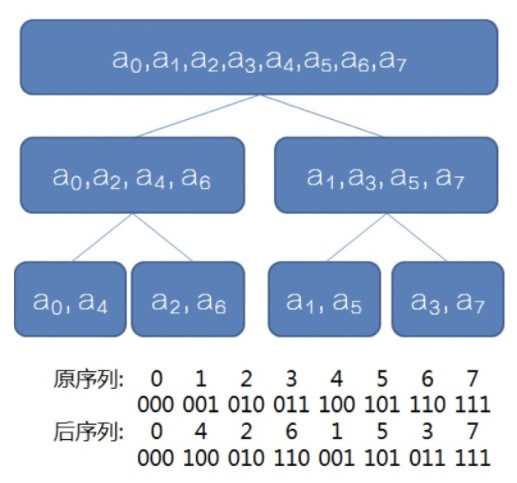
\includegraphics[width=0.5\textwidth]{GPU-The butterfly networks of Cooley-Tukey NTT.jpg}
    \caption{The butterfly networks of Cooley-Tukey NTT}
    \label{fig:The Butterfly Networks of Cooley-Tukey NTT}
\end{figure}
\subsubsection{2-D NTT}
NTT is an important kernel commonly used in our ZK scheme. In fact, there exist many accelerator designs for NTT. However, the polynomial computations in our ZK scheme have substantially larger scales than those addressed in other ZK. It requires multiple NTTs of up to $2^{23}$ or $2^{24}$ elements, Such large sizes can hardly be satisfied by any previous GPU design.

To overcome the large-sizes challenges, we adopt a 2-D NTT algorithm to decompose a large NTT into multiple smaller NTT kernels (4096/8192). This allows GPU to only implement smaller NTT modules, which can fit into the compute resources (e.g. the stream processor number of on GPU). Then the original large-size NTT can be calculated by iteratively using the smaller NTT.

The overview of 2-D NTT algorithm is shown in \figref{fig:The 2-D NTT Algorithm}. First of all, a large NTT size N is decomposed into P rows and Q columns, with $N=P \times Q$. Then the N-size NTT can be calculated by several P-size and Q-size smaller NTTs. Firstly, the P-size NTT is parallel computing using the same twiddle factors for each of the Q columns. The output is still a P-size vector. Before the second dimensional NTT, a corresponding twiddle factor $\omega^{ij}$ is multiplied to each element of the output vector. Finally, a Q-size NTT for each of the P rows is parallel computing. The output column-major order elements is the result of the large-size NTT.
\begin{figure}[!ht]
    \centering
    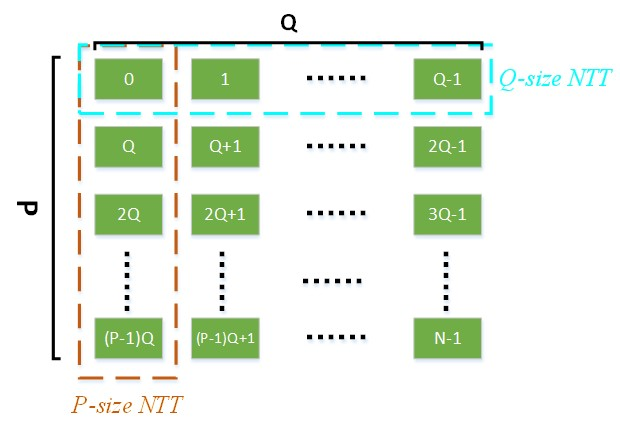
\includegraphics[width=0.6\textwidth]{GPU-The 2-D NTT algorithm.jpg}
    \caption{The 2-D NTT algorithm}
    \label{fig:The 2-D NTT Algorithm}
\end{figure}
\subsubsection{GPU and CUDA}
Currently, the GPU is no longer limited to graphics processing. Thanks to the rapid evolution of their architecture that made it straightforward to access their underlying powerful  parallelism to address different categories of data parallel algorithms to be handled efficiently by this platform. The GPU is designed to process a huge amount of numbers operations in parallel relying on thousands of computing cores running concurrently. CUDA is a general-purpose parallel computing architecture that delivers a novel parallel programming paradigm and a new instruction set architecture that can easily leverage the parallel power of the computing engine embedded in the CUDA-enabled GPUs to solve complex scientific and engineering applications. It becomes straightforward to decompose the computations into fine-grained threads and execute theses threads on the device in parallel. CUDA refers to the software platform and the hardware architecture used to execute the kernels. A kernel launches thousands of threads for parallel execution organized in three levels: grids, blocks, and warps. The grids are two- or three-dimensional arrangements of threads blocks where every block consists of an upper limit of threads 512 or 1024 depending on the compute capability version of the device, and finally each group of threads form a wrap. Such architecture is called Single Instruction Multiple Thread (SIMT); which allows the GPU to execute single instruction on multiple concurrent threads operating on different data. Every running thread has access to some built-in variable assigned by the CUDA run time system and used for thread indexing. CUDA also has an efficient memory hierarchy divided in global, shared, register, texture, and constant memory.
\subsubsection{Implement of 2-D NTT with GPU}
To overcome the large-sizes challenges on GPU, the 2-D NTT algorithm is adopted. For a particular GPU model, the number of stream processors has been set to a fixed value, so the total number of threads running simultaneously on this GPU is limited. In order to make full use of the GPU thread resources, we set NTT's two-dimensional running framework as shown in \figref{fig:Implement of 2-D NTT with GPU} with a $2^{23}$ size NTT. The NTT sequence is divided into 8192 rows and 1024 columns. For each column, 8192 threads (This number can be adjusted based on the number of stream processors to achieve maximum GPU utilization) are allocated to calculate 8192-size 1D NTT in parallel.
\begin{figure}[!ht]
    \centering
    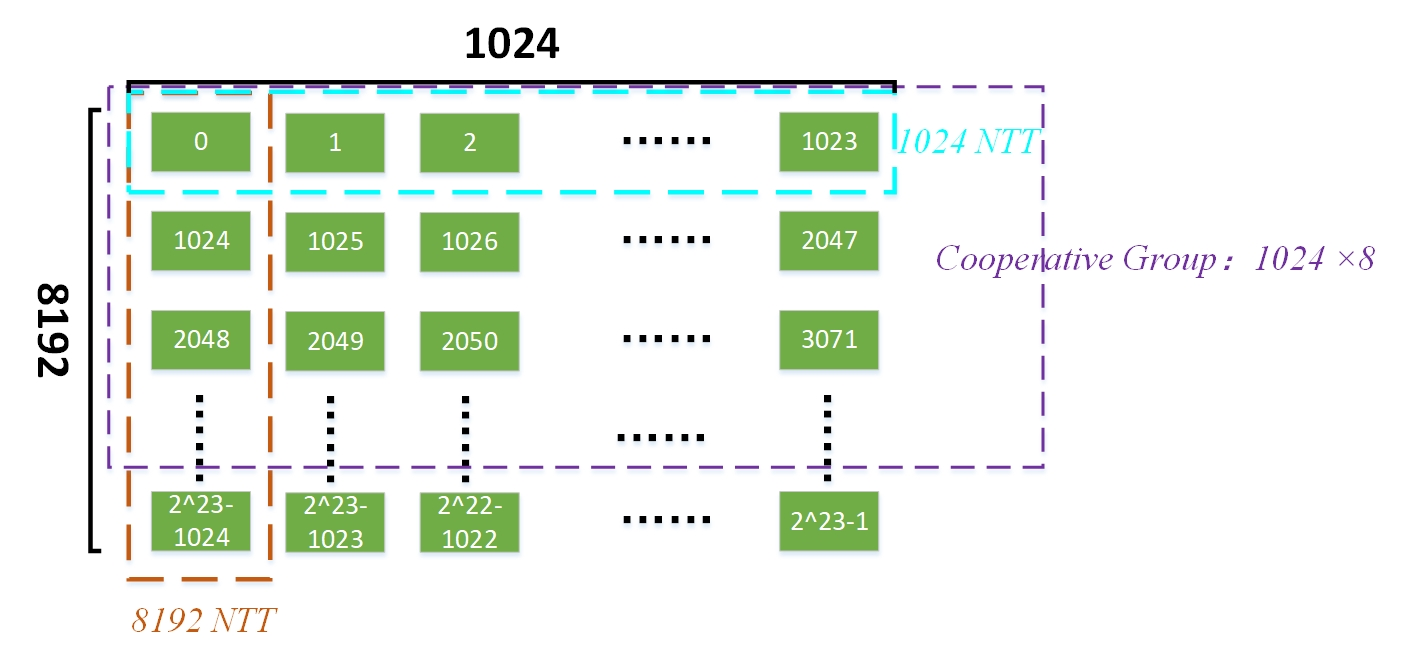
\includegraphics[width=0.7\textwidth]{GPU-Implement of 2-D NTT with GPU.jpg}
    \caption{Implement of 2-D NTT with GPU}
    \label{fig:Implement of 2-D NTT with GPU}
\end{figure}
After processing each column, the NTT of the second dimension can process 8 rows at a time through the Cooperative Groups (CG) mechanism. The Cooperative Groups programming model describes synchronization patterns both within and across CUDA thread blocks. It provides CUDA device code APIs for defining, partitioning, and synchronizing groups of threads. It also provides host-side APIs to launch grids whose threads are all guaranteed to be executing concurrently to enable synchronization across thread blocks. These primitives enable new patterns of cooperative parallelism within CUDA, including producer-consumer parallelism and global synchronization across the entire thread grid or even multiple GPUs.

Therefore, the total running time of the GPU is 1024 8192-size NTTs plus 1024 1024-size NTTs.
\subsubsection{Memory Access}
The following \figref{fig:CUDA Memory Model} shows the CUDA memory model. The large-size NTT data is copied from the host into global memory. Then it is sent to shared memory into the compute queue. For faster access, precomputed twiddle factors are stored in texture memory. When the twiddle factor is used, it is copied sequentially to the registers according to the index. The results of one-dimensional NTTs are saved in shared memory. When the NTT is calculated, the output is copied from shared memory to global memory and uploaded to the host.
\begin{figure}[!ht]
    \centering
    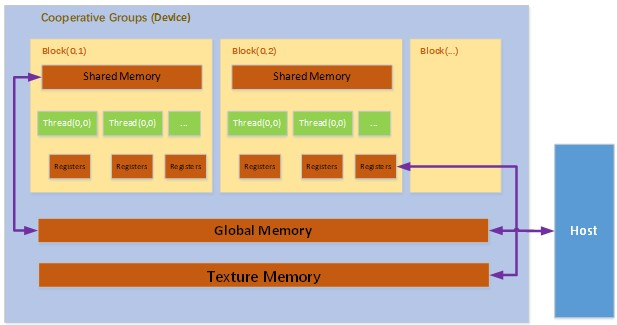
\includegraphics[width=0.7\textwidth]{GPU-CUDA memory model.jpg}
    \caption{CUDA Memory Model}
    \label{fig:CUDA Memory Model}
\end{figure}
